%%%%%%%%%%%%%%%%%%%%%%%%%%%%%%%%%%%%%%%%
%% MCM/ICM LaTeX Template %%
%% 2020 MCM/ICM           %%
%%%%%%%%%%%%%%%%%%%%%%%%%%%%%%%%%%%%%%%%
\documentclass[12pt]{article}
% \documentclass{article}
\usepackage{geometry}
\geometry{left=1in,right=0.75in,top=1in,bottom=1in}

%%%%%%%%%%%%%%%%%%%%%%%%%%%%%%%%%%%%%%%%
% Replace ABCDEF in the next line with your chosen problem
% and replace 1111111 with your Team Control Number
\newcommand{\Problem}{\textcolor{cyan}{REPLACE ME WITH PROBELM}}
\newcommand{\Team}{\textcolor{cyan}{REPLACE ME WITH TEAM NUMBER}}
%%%%%%%%%%%%%%%%%%%%%%%%%%%%%%%%%%%%%%%%

% \usepackage{newtxtext}
\usepackage{amsmath,amssymb,amsthm}
% \usepackage{newtxmath} % must come after amsXXX

\usepackage[pdftex]{graphicx}
\usepackage{xcolor}
\usepackage{fancyhdr}
\usepackage{setspace}
\usepackage{graphicx}
\usepackage{float}
\usepackage{subcaption}
% This is gonna give you footnote
% \usepackage[backend=bibtex,style=verbose-trad2]{biblatex}
% And this is gonna give you some collection
\usepackage[backend=bibtex,style=ieee]{biblatex}
\usepackage{siunitx} % Required for alignment
\usepackage{multirow}
\usepackage{booktabs} % For prettier tables
\usepackage{longtable} % To display tables on several pages
\usepackage{rotating} % To display tables in landscape
\usepackage{pgfplotstable} % Generates table from .csv
\usepackage{tikz}
\usepackage{pgfplots}
\usepackage{csvsimple}
\usepackage{listings}
\usepackage[utf8]{inputenc}
% Well guess you need this to make sure line break of minted listing is working fine
\usepackage[newfloat]{minted}
% \usepackage{caption}
\usepackage{pgf}
\usepackage{import}
\usepackage{pdfpages}
\bibliography{summary}


\lhead{Team \Team}
\rhead{}
\cfoot{}

\newtheorem{theorem}{Theorem}
\newtheorem{corollary}[theorem]{Corollary}
\newtheorem{lemma}[theorem]{Lemma}
\newtheorem{definition}{Definition}

%%%%%%%%%%%%%%%%%%%%%%%%%%%%%%%%
\begin{document}
\graphicspath{{.}}  % Place your graphic files in the same directory as your main document
\DeclareGraphicsExtensions{.pdf, .jpg, .tif, .png}
\thispagestyle{empty}
\vspace*{-16ex}
\centerline{\begin{tabular}{*3{c}}
        \parbox[t]{0.3\linewidth}{\begin{center}\textbf{Problem Chosen}\\ \Large \textcolor{red}{\Problem}\end{center}}
         & \parbox[t]{0.3\linewidth}{\begin{center}\textbf{2020\\ MCM/ICM\\ Summary Sheet}\end{center}}
         & \parbox[t]{0.3\linewidth}{\begin{center}\textbf{Team Control Number}\\ \Large \textcolor{red}{\Team}\end{center}} \\
        \hline
    \end{tabular}}
%%%%%%%%%%% Begin Summary %%%%%%%%%%%
% Enter your summary here replacing the (red) text
% Replace the text from here ...
\begin{center}
    \textcolor{red}{%
        Use this template to begin typing the first page (summary page) of your electronic report. This \newline
        template uses a 12-point Times New Roman font. Submit your paper as an Adobe PDF \newline
        electronic file (e.g. 1111111.pdf), typed in English, with a readable font of at least 12-point type.	\\[2ex]
        Do not include the name of your school, advisor, or team members on this or any page.	\\[2ex]
        Papers must be within the page limit specified in the problem statement.	\\[2ex]
        Be sure to change the control number and problem choice above.	\\
        You may delete these instructions as you begin to type your report here. 	\\[2ex]
        \textbf{Follow us @COMAPMath on Twitter or COMAPCHINAOFFICIAL on Weibo for the \newline
            most up to date contest information.}
    }
\end{center}
% to here
%%%%%%%%%%% End Summary %%%%%%%%%%%

%%%%%%%%%%%%%%%%%%%%%%%%%%%%%%
\clearpage
\pagestyle{fancy}
% Uncomment the next line to generate a Table of Contents


\begin{center}
    \Large \textbf{Kingdom Built on a Pile of Sand:Slow and Steady}
\end{center}

\newpage

\tableofcontents
\newpage
\setcounter{page}{1}
\rhead{Page \thepage\ }

\section{Introduction}
\subsection{Problem Background}
\par
Sunshine, clear blue sea and golden color sand always seem to leave people in a happy state of mind.
And a beach is where these three are combined, drawing people all around towards it. Sand, the granular matter formed by constant brushing of flowing water, however, can react with water in a different way, despite the fact that people refer to it as non-stable or unreliable. On a beach, where the already formed granular sand and the rise and fall of sea wave lies together, a new buff can be added to our flowing friend, a wetted state.
\par
Magically but not randomly, sand gets sticky when combined with water, due to the most obvious physical theorem: surface tension and atmosphere pressure. From previous people's work, we've know that this buff comes from the water bridge formed between sand particles, which can significantly cluster together during the increasing water-sand portion\autocite{pakpour2012construct,mitarai2006wet,kudrolli2008sticky}. Kudrolli and Arshad has visualized the bridge between sand like Figure \ref{fig:water_bridge}.
\par
<<<<<<< HEAD
And that's the magic that glue our favorite sand castle together, which is one of the most entertainment for enthusiastic beach goers. However, being built near the water that melts mud and our wet sand, all sand castles have to face the fate that they'll get too wet to hold its own weight and the impact from sea waves. That's because the water bridge has another property of clustering together\autocite{kudrolli2008sticky}. When you throw a pile of sand into water, they behave just as when they're completely dry, melting down like fluid. Thus beach castle builder might want to make their sand castle last longer than those build arbitrarily than others, which is also the purpose of this article.
=======
And that's the magic that glue our favorite sand castle together, which is one of the most entertainment for enthusiastic beach goers. However, being built near the water that melts mud and our wet sand, all sand castles have to face the fate that they'll g et too wet to hold its own weight and the impact from sea waves. That's because the water bridge has another property of clustering together\autocite{kudrolli2008sticky}. When you throw a pile of sand into water, they behave just as when they're completely dry, melting down like fluid. That is, sand castles lasts for only a period of time. Thus beach castle builder might want to make their sand castle last longer than those build arbitrarily than others, which is also the purpose of this article.

>>>>>>> 41791c65690afc4c2eb94bdef0ba84e26bfc9b6b

\begin{figure}
    \centering
    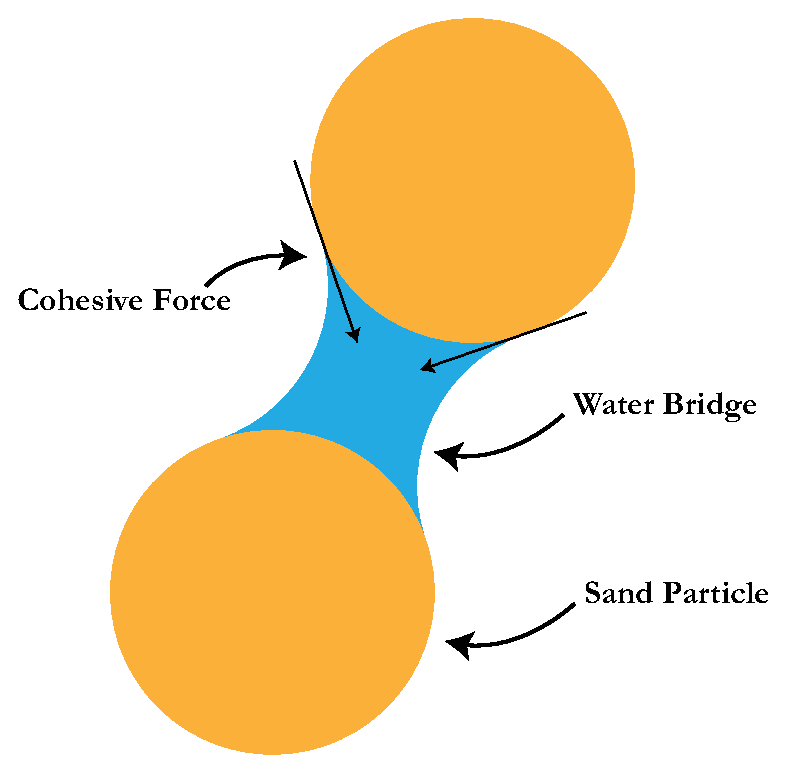
\includegraphics[width=0.5\linewidth]{water_bridge.eps}
    \caption{Water Bridge Between Sand Particle}
    \label{fig:water_bridge}
\end{figure}

\subsection{Our Work}
Normally people would sculpt their kingdom from a pile of tedious wet sand. To simplify the model and grasp main threads, we'll focus our research on this single, nondescriptive mound of wetted sand. In this article, we develop a method for determining the most long-lasting three dimensional shape for a tedious sand castle, which will be later referred to as \textit{sand castle foundation}.
\par
Our model addresses the problem of constructing a three dimensional structure by projection, which makes the construction of individual part of our model easy to implement. Firstly we determine the optimal \textit{side view} of our \textit{sand castle foundation} by analysing and extracting information from similar research on wet granular material\autocite{mitarai2006wet}. Then we construct the best \textit{top view} of the \textit{sand castle foundation} by constructing a \textbf{Cellular Automata}.

\paragraph{Side Slope Determination}
You've probably seen questions about the slope of a pile of dry sand in junior high school practice books. In our research, we address the problem about dry sand as a normal junior high student would. However, the analysis of wet sand requires some technique beyond low level physics. In our research, we establish this model using \textbf{Mohr-Coulomb Criterion}.

\paragraph{Top View Determination}
Our model analyses the impact of sea wave flow from a top view, or a \textit{slice} of the \textit{sand castle foundation}. Then we can combine the sliced impaction result together with the \textit{side slope} analysis to form a possible 3D object. Inside our model we construct a \textbf{Cellular Automata} since the shape of the sand slice edge isn't as obvious the side slope may be, that is, it's merely possible to construct continuous function on the shape.

\paragraph{Other Factors}
It's worth noting that the interaction between sand and sea wave is far a lot more complex than direct force impact or sand-to-water mixture proportion change. Some other factors include: gravity of sea water that submerge the sand underneath, influx of weaker sea wave and the gravity of water inside the wetted sand. During the assembly of two views, we'll address these other factors that may influence a \textit{sand castle foundation}'s life span.

\section{Assumptions \& Nomenclature}
\subsection{Assumptions}
Several assumptions are made in order to simplify our model.
\begin{itemize}
	\item [1)] 
	The weather condition is suitable for sand castle building, namely, there is no wind and...
	\item [2)]
	The height of wave is the same, which we set as...
	\item [3)]
	Our optimization goal is to acquire the largest top size while minimizing the lost of sand. Intuitively, if the side of the foundation is built as a gentle slope, the possibility of collapsing will be drastically reduced. However, with a fixed volume of sand, such a foundation will not allow any sophisticated carving.
	\item [4)]
	Sand grains are regarded as tiny spheres. In our foundation, these grains are of the same size and are closely packed. 
	\item [5)]
	The top of the foundation is a flat platform whose surface is horizontal.
	\item [6)]
	...
\end{itemize}
\subsection{Nomenclature}
\begin{table}[H]
	\caption{States of Sand}
	\vspace{5pt}
	\centering
	\begin{tabular}{p{3cm}p{12cm}}
		\hline
		Symbol & Meaning \\
		\hline
		$\tau$   & the shear stress on a plane \\
		$\tau_f$ & the shear stress on the failure plane\\
		$\mu$    & the internal friction coefficient \\
		$\sigma$ & the normal compressible stress on a plane \\
		$\sigma_f$ & the normal compressible stree on the failure plane \\
		$\rho$   & the density of sand \\ 
		$\theta_c$ & the critical angle of a sandpile\\
		$D$ & the height from the top of the sand pile \\
		$P$ & the pressure[] \\
		$\Gamma$ & the surface tension of water \\
		$s_A$ & the adhesive stress \\
		$f_A$ & the adhesive force \\
		$V$ & the total amount of fluid present per particle contact \\
		$R$ & the radius of particle \\
		\hline       
	\end{tabular}
	\label{bs2}
\end{table}


\section{Modeling Under Waves and Tides}

\par
<<<<<<< HEAD
The 3-dimensional shape constructing problem is divided into two subproblems. We first establish the model using the \textbf{Mohr-Coulomb Criterion} to decide the shape of the slope. We then construct another model with a modified version of \textbf{a modified version of Cellular Automata} to determine the best shape viewed from the top,...
=======
The 3-dimensional shape constructing problem is divided into two sub-problems. We first establish the model using the \textbf{Mohr-Coulomb Criterion} to decide the shape of the slope. We then construct another model with a modified version of \textbf{Cellular Automata} to determine the best shape viewed from the top,...
>>>>>>> 41791c65690afc4c2eb94bdef0ba84e26bfc9b6b

\subsection{Shape of the Slope: Mohr-Coulomb Criterion}


We begin by determining the side shape of the sand castle foundation. Before Approaching the problem, we will briefly address the property of sand as a granular media.
\par
In our assumptions, sand particles are considered as identical tiny spheres. If we zoom in to observe a pile of wet sand, there are the so-called liquid bridges formed between sand particles.
\par
Various water contents produce different liquid bridge distributions, which will influence the properties of sand.

\begin{table}[H]
	\caption{States of Sand}
	\vspace{10pt}
	\centering
	\begin{tabular}{p{4cm}p{2cm}p{4cm}p{4cm}}
		\hline
		Liquid Content & State & Description & left for future use \\
		\hline
		No  			  & Dry   	    & 000          & 000                    \\
		Small  			  & Pendular    & 000     	   & 000                        \\
		Middle  		  & Funicular   & 000    	   & 000                        \\
		Almost saturated  & capillary & 000          & 000                        \\
		More  			  & Slurry      & 000          & 000                        \\  
		\hline       
	\end{tabular}
	\label{bs2}
\end{table}
\par
When the wave gets into contact with the foundation, the surface area is in slurry state and there exists no cohesive interaction between the particles, which makes it very hard, if not impossible, to prevent sand loss. Nevertheless, collapses after the wave resides can cause more harm to the foundation, which can be avoided by alternating the shape.
\par 
For dry sand, the failure criterion is given in terms of the shear stress $\tau$, the normal compressible stress $\sigma$ and the internal friction $\mu$ as
$$\tau > \mu\sigma$$
This is simply the friction formula with different notations. For wet sand, we consider a sandpile with a normal adhesive stress $s_A$ across every plane, in addition to the stress caused by weight. The equation(1) is then modified as
$$\tau > \mu(\sigma + s_A)$$
This is the so-called \textbf{Mohr-Coulumb criterion}. The stress resulting from the weight above the plane is shown in figure(2). Denote $\tau_f$ and $\mu_f$ as the shear stress and normal compressible stress at the failure plane, it is obvious from the schematic that they can be written as
$$\tau_f = \rho gDsin\theta_c \qquad and \qquad \sigma_f = \rho gDcos\theta_c$$
where $\theta_c$ is the critical angle, $D$ is the height of the sandpile and $\rho$ is the density of sand. Therefore, combine the equations above, to solve for $\theta_c$ is to solve the equation
$$\mu = tan\theta_c(D)\bigg(1 + \frac{s_A}{\rho gDcos\theta_c(D)}\bigg)$$
\par
The only unknown factor is $s_A$, the adhesive stress across the plane. According to (Thomas C.H and Alex J.L -fix later)'s study, the value of $s_A$ is determined by water content and there are three regimes as a function of the added-fluid volume. We now focus only on the state where the water content is close to saturation. 
\par
In this case, with water serves as lubricate, it makes sense to model sand particles as frictionless spheres. The pressure difference is then given by [] 
$$P = -\frac{\Gamma}{\sqrt{V/2\pi R}}$$
where $\Gamma$ is the surface tension of the fluid, V is the total amount of fluid present per particle contact, and R the radius of the particle. The adhesive force is given by
$$f_A = 2\pi \Gamma R$$
Note that (with certain conditions like distance between grains remains constant)the term $V$ which denotes the volume of liquid does not appear in equation(6).
\par
Assume our foundation contains sand particles that are closely packed. Such structure means there is an average of 6 contacts per square.

\subsection{Top View Shape}
\par 
We used a modified version of\textbf{ cellular automata} to simulate the impact of tides and waves. There are several factors that are taken into consideration:
\par 
\begin{itemize}
	\item [1)] 
	...     
	\item [2)]
	...
	\item [3)]
	...
\end{itemize}

\begin{figure}[H]
	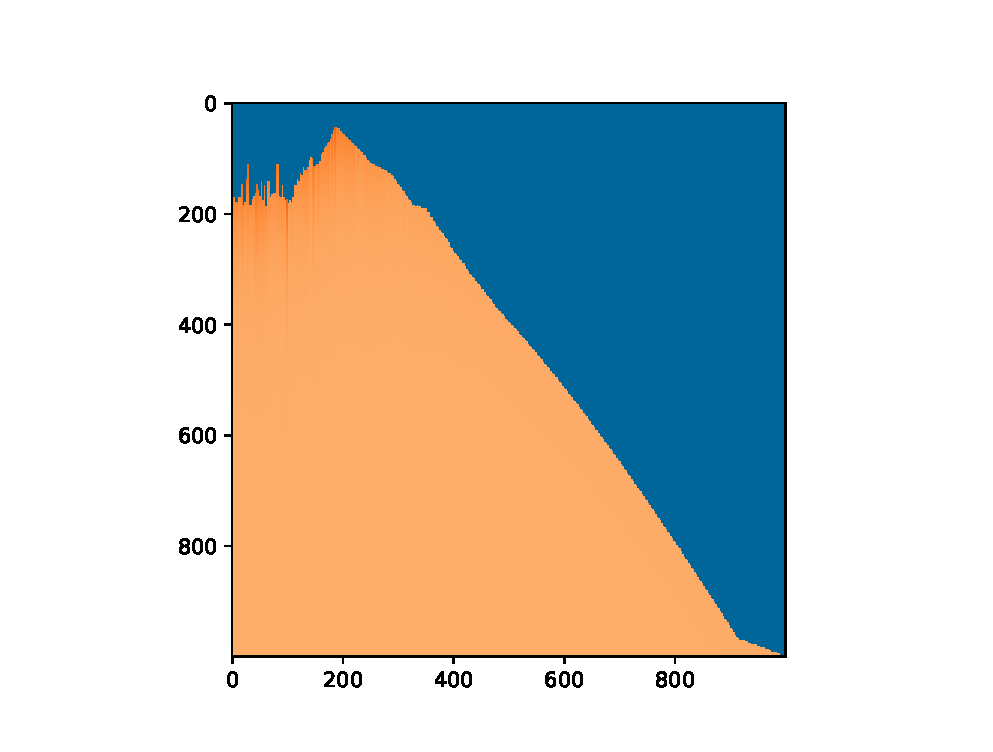
\includegraphics[width=\linewidth]{Figure_1.eps}
	\caption{A Windows Terminal.}
	\label{fig:Terminal}
\end{figure}
\textcolor{cyan}{This is a test figure. Remember to delete me.}
\begin{figure}[H]
	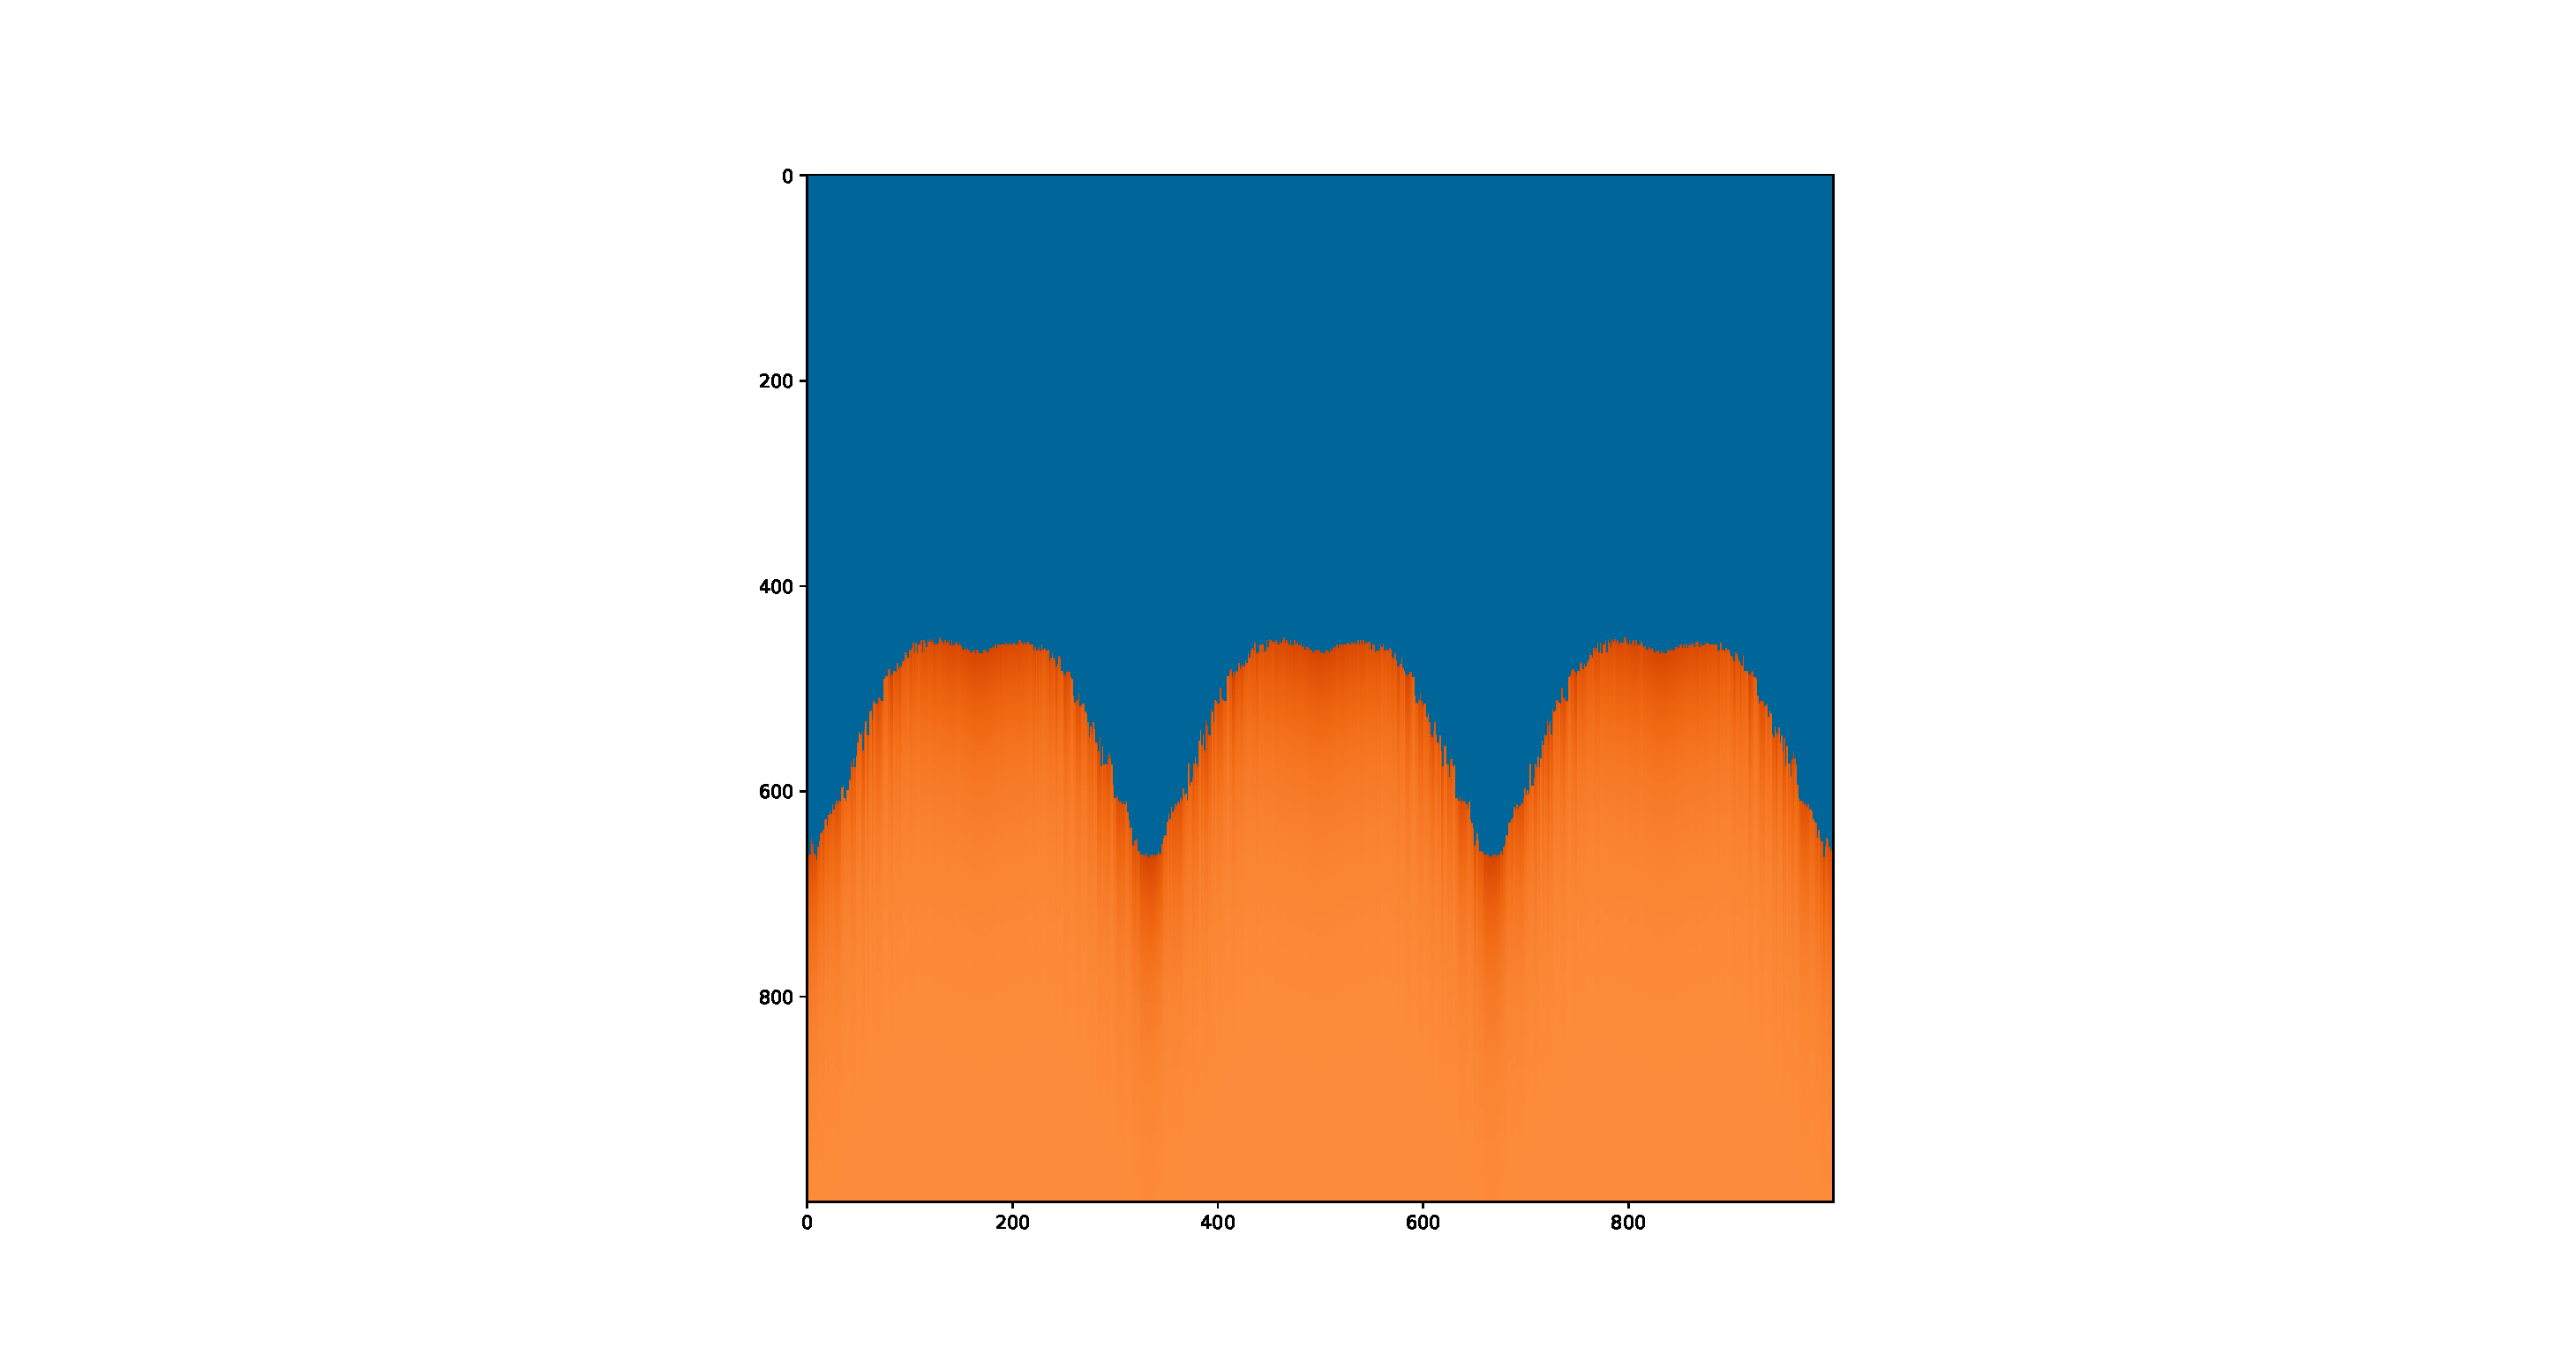
\includegraphics[width=\linewidth]{Figure_2.eps}
	\caption{A Windows Terminal.}
	\label{fig:Terminal}
\end{figure}
\subsection{Calculate \& Simulate Results}
Briefly review the equation derived in section 3.1
$$tan\theta_c = \mu + \frac{\sqrt{2}\pi\mu\Gamma}{R\rho gD}sec[tan^{-1}(k)]$$
To solve for the best shape of the slope, the necessary information about sand is listed below
\begin{table}[H]
	\caption{States of Sand}
	\vspace{10pt}
	\centering
	\begin{tabular}{p{4cm}p{2cm}p{2cm}}
		\hline
		Physical Quantities & Values & Units 	\\
		\hline
		$\Gamma$		  & 72.8   	    & $mN/m$              \\
		$\mu$  			  & 0.55~0.60   & -     	            \\
		$\rho$ 			  & 1631     &  $kg/m^3$          \\
		$R$ 			  & 0.05~2   & $mm$               \\
		$g$  			  & 9.81      & $m/s^2$     \\
		\hline
	\end{tabular}
	\label{bs2}
\end{table}
\par
It is not sensible to embark on a trip to the beach on a stormy day, so we assume that the near-shore wave is gentle, with its height not exceeding 20cm, or $D \in [0, 20](unit:cm)$.
We first assume that..

\section{Modeling Under Rain}

\section{Determine the Best Sand-to-water Proportion}
\section{Other Ways to Make Our Sand Castle Last Longer}
\subsection{Dig a Moat}
Building a moat can help our sand castle foundation to survive the rising tide. 
\subsection{Make It Compact}
There are two advantages of making a compact foundation.
\paragraph{More Contact Points}
\paragraph{Fewer Cracks}
\subsection{Further From the Shore}
According to our analysis in section 5, the optimal sand-to-water proportion is 1\%. 
(This is not possible if the castle can be reached by wave...)
\subsection{Finer Sand}
Finer sand is a bonus because by constructing our sand castle foundation using it, the foundation has a greater critical angle. That is because the term $R$, which is a part of the denominator, decreases and (enlarge?not the proper word) the value of $tan\theta_c$. 
\subsection{Special Material}
\paragraph{Glue}
Sand sculptures seen in exhibitions or competitions have their surfaces covered with special glue. The glue is mainly used protect the sand sculpture from drying out or crumbling if the waves do not wash it away first, but it also keeps water out. In our model where the greatest enemy of the foundation is not collapses but erosion, such glue will help maintain the shape of the foundation. 
\paragraph{Mixture}
Concrete, a material that everyone is familiar with, has sand as its ingredient. 
\section{Sensitivity Analysis}
\subsection{Model Under Waves and Tides}
\paragraph{Side View Shape}
Here, insert the schematics I drew. They are far from perfect but they ARE a part of sensitivity analysis.
\paragraph{Top View Shape}
DenDen dl has done a lot of parameter adjusting jobs...those are exactly what we need here.
\subsection{Model Under Rain}
Not now. Wait for tomorrow or something.
\section{Strengths and Weaknesses}
\subsection{Strengths}
Just like any other model, the one presented above has its Strengths and Weaknesses. Some major points are listed below.
\begin{itemize}
	\item [1)] 
	The use of Cellular Automata enables our model to predict erosion of any possible shape. 
	\item [2)]
	
	\item [3)]
	...
\end{itemize}
\subsection{Weaknesses}
\begin{itemize}
	\item [1)] 
	Our model in section 3.1 does not consider the impact of the wave, which...  
	\item [2)]
	...
	\item [3)]
	...
\end{itemize}

\textcolor{cyan}{This is a test figure. Remember to delete me.}



This is some example text\footnote{\label{myfootnote}Hello footnote}.

I'm referring to footnote \ref{myfootnote}.


\newpage
\begin{appendix}
    \listoffigures
    \listoftables
    \listoflistings
    % \bibliographystyle{ieeetr}
    \printbibliography
\end{appendix}
\end{document}
